% !TeX root = ../thuthesis-example.tex

\chapter{简介}

\section{历史背景}

\begin{figure}[htb]
	\centering
	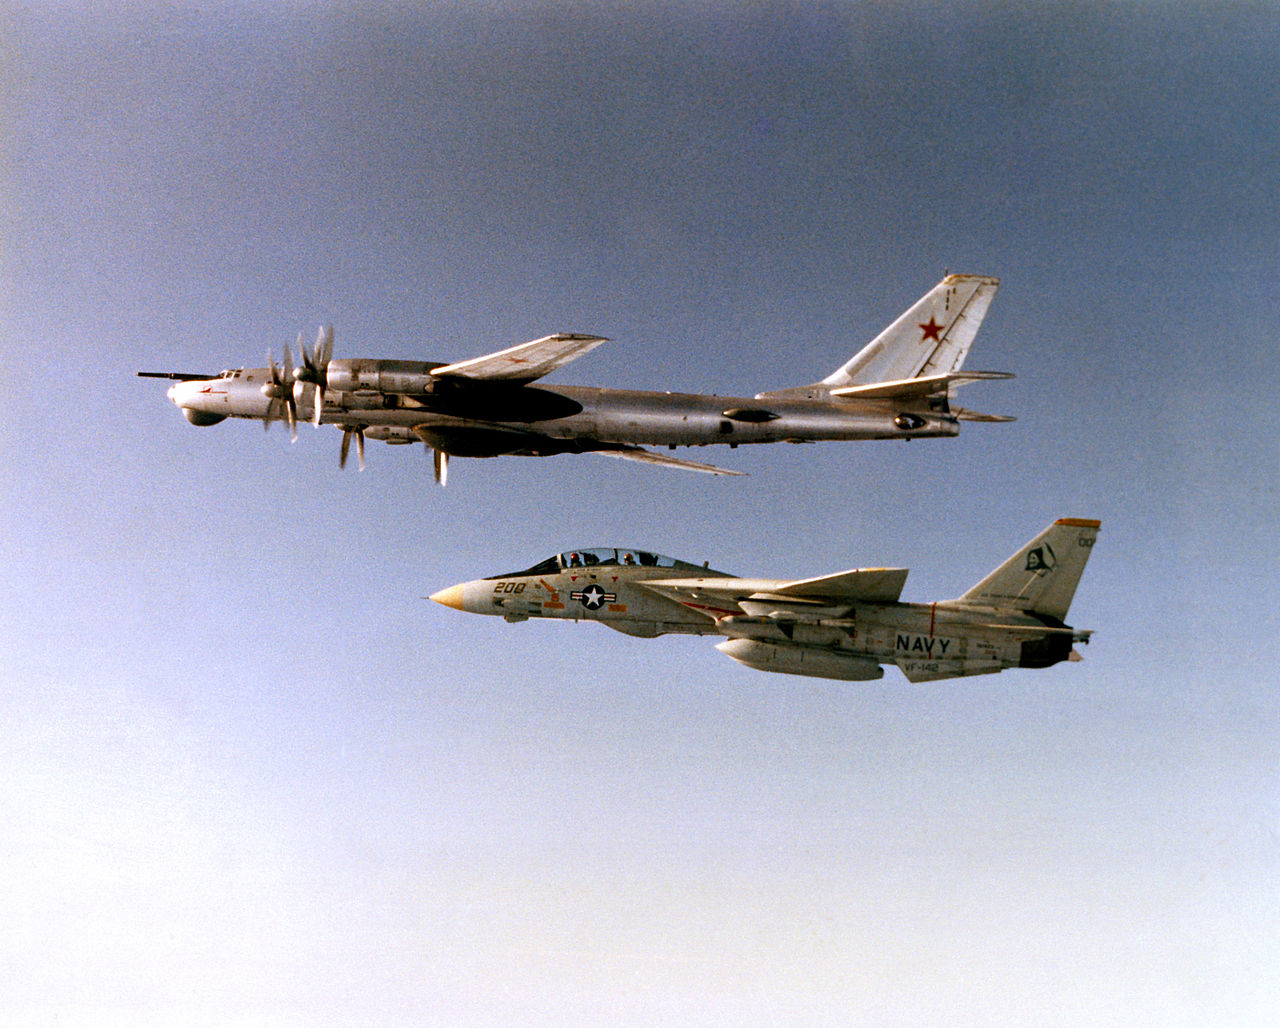
\includegraphics[width=0.6\textwidth]{F-14TU95.png}
	\caption{照片由美国海军中尉Thomas Prochilo拍摄(DN-SC-83-06680)}
\end{figure}

F-14“雄猫”可以一直追溯到上世纪50年代,美国海军急需一架长航程舰载截击机来填补舰队防空职能的空缺。结论认为海军需要一架比 F-4“鬼怪”更先进、雷达探测距离更远、空空导弹射程更长的战斗机。

当时,海军受国防部长罗伯特·麦克纳马拉的指示与美国空军合作推进实验战术战斗机(TFX)项目。海军从最初便反对共同开发此项目,而且通用动力F-111B飞机方案也并未满足海军的期望。

和通用动力共同开发海军 F-111B 而加入 TFX 项目的格鲁曼公司最终获得了海军制定的更符合自身情况的舰载机研发合同。装备着沿用失败的 F-111B 项目的雷达(AN/AWG-9)和导弹(AIM-54“不死鸟”)的 F-14 战斗机便从这份研发合同中诞生了。

F-14“雄猫”于1970年12月21日首飞,并于1974年9月22日开始服役。“雄猫”(Tomcat)这个名字一方面遵循格鲁曼用猫科动物命名飞机的传统,另一方面也源于海军中将Thomas F. Connolly的昵称“Tom's Cat”(“汤姆的猫”),以纪念他对F-14研发所做的关键贡献。

\subsection{服役升级}

F-14A是F-14战斗机的第一个型号,配备普惠TF30发动机并在机鼻下方的吊舱中装备了IRST系统。

对 F-14A 而言,TF30 发动机的稳定性和动力常常不尽人意。于是在 F-14A+(后来的 F-14B )上,TF30发动机被通用电气 F110-400 发动机所取代。

F-14A 的 IRST 系统也表现不佳并很快被 TCS(电视摄像机组件)吊舱所取代。TCS 吊舱允许飞行员对雷达追踪目标进行超视距目视识别。

F-14A 和 F-14B 在服役期间都得到了持续升级,包括新的可编程座舱显示器(PTID 和 PMDIG),以及新的 INS 惯导系统、数字飞控系统(DFCS)和 RWR 系统等。

最终,TARPS(战术空中侦察吊舱)系统的装备使 F-14 获得了收集影像资料进行战术侦查任务的能力。

\subsection{对地攻击}

\begin{figure}[htb]
	\centering
	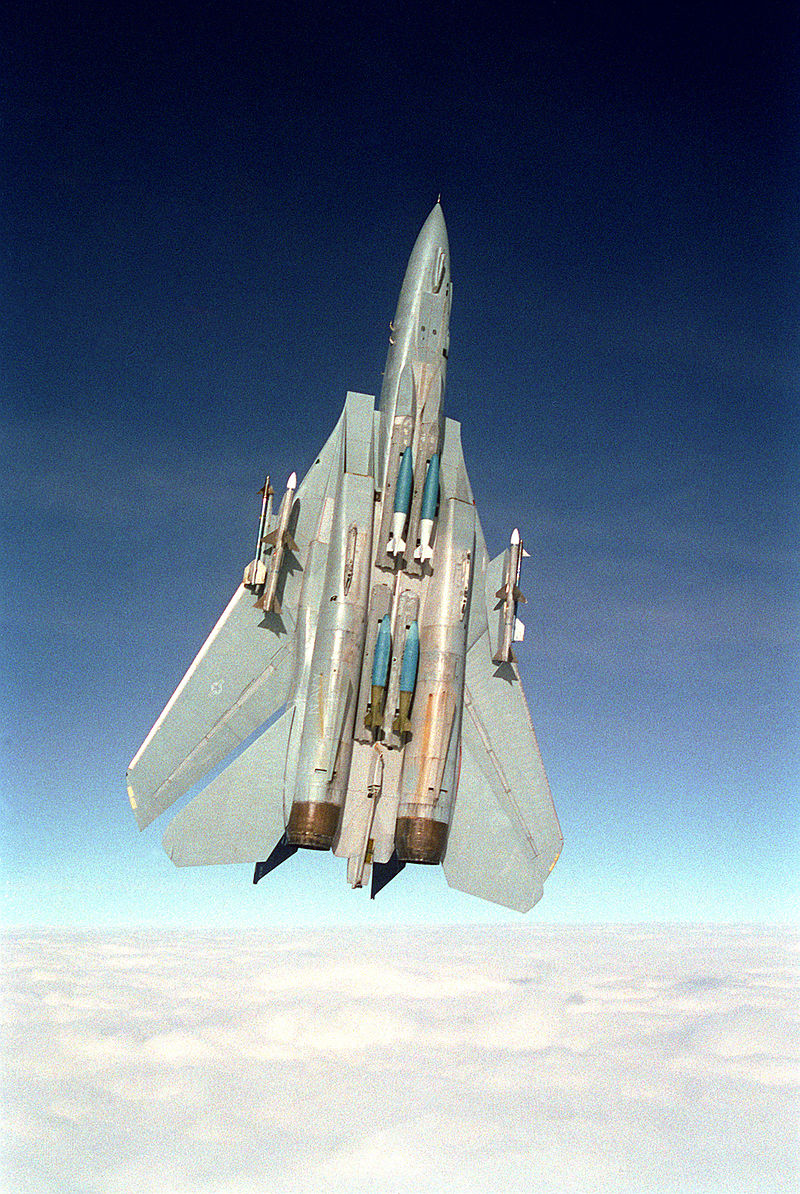
\includegraphics[width=0.6\textwidth]{bombcat.png}
	\caption{照片由美国海军少校 Dave Parsons 拍摄 (DN-SC-93-01299)}
\end{figure}

20世纪90年代,美国海军舰队面临的空中威胁逐渐减少,同时由于沙漠风暴等行动的实施,对地攻击的重要性重新凸显出来。

F-14 最初就具备携带和投放空对地弹药的能力,但是由于海军基于成本和风险的考量,F-14 的主要职责仅为舰队防空。

随着任务角色的转变,一些 F-14A 和 F-14B 开始挂载 LANTIRN 目标吊舱以便 RIO 为自己和其他飞机搜索目标、引导激光制导炸弹。 随后,F-14 还增加了携带和投放 GPS 制导的 JDAM 弹药的能力。

大部分装备了 LANTIRN 吊舱的 F-14 都升级了可编程 TID(PTID)以更好地集成 LANTIRN 吊舱的功能。

\subsection{F-14D}

20世纪90年代,F-14 的终极型号 F-14D 开始服役。

F-14D 使用和 F-14B 同样的 GE F110-400 发动机,同时也装备了数字飞控系统(DFCS)。DFCS 系统随后也开始装备在较老的在役 F-14A 和 B 型上。

此外,F-14D 还安装了 AN/AWG-9 雷达的改进型,AN/APG-71 雷达以及一整套升级的航电系统。原本的 TCS 吊舱也升级成了一个融合了改进版 IRST 系统与 TCS 功能的新吊舱。

\subsection{退役}

F-14“雄猫”最终还是老态龙钟了。随着维护成本的增加和机体的老化,海军不得不开始退役“雄猫”。冷战的结束也使得“雄猫”的本职——舰队防空显得不那么重要了。

2006年9月22日,最后一架雄猫的退役仪式在欧希安纳海军航空站举行。

\subsection{伊朗}

\begin{figure}[htb]
	\centering
	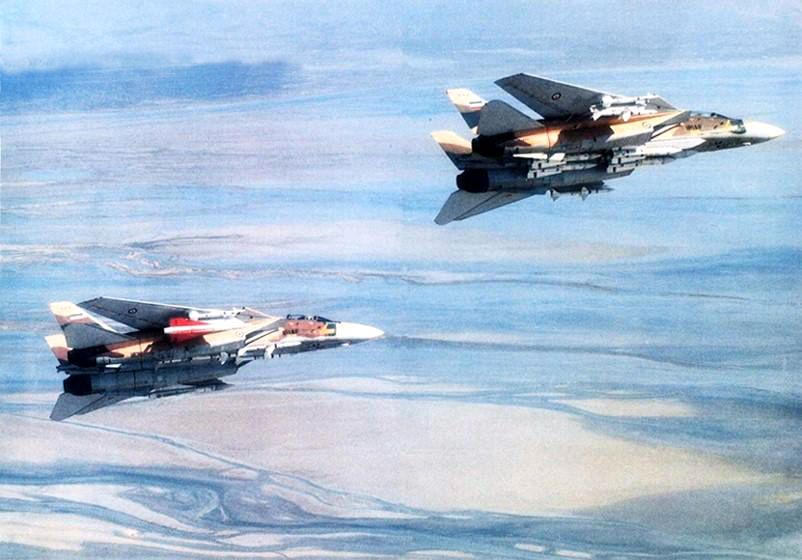
\includegraphics[width=0.6\textwidth]{iranicats.jpg}
	\caption{照片由伊朗空军在1986年间拍摄}
\end{figure}

F-14“雄猫”的唯一海外使用客户是伊朗皇家空军(IIAF)和后来的伊朗伊斯兰共和国空军(IRIAF)。当时的伊朗国王默罕默德·礼萨·巴列维曾采购了80架“雄猫”。

而巴列维王朝的倒台和伊朗伊斯兰共和国的崛起意味着一个反美国家获得了美国最先进的战斗机之一。“波斯猫”随即失去了所有零部件和导弹的供应,只得从黑市上购买配件,这大大增加了飞机维护的难度。

伊朗在两伊战争期间使用了 F-14“雄猫”并声称取得了大量对伊拉克空军的空中胜利。小道消息称当时伊拉克飞行员甚至会为了避开 AN/AWG-9 和 AIM-54 的威胁而逃离交战空域。

目前为止,只有伊朗共和国空军还在使用 F-14“雄猫”。目前伊朗人获得飞机配件的途径还不明确,有推测认为他们通过拆除无法飞行的飞机上的零件来维持机队其他飞机的状态。还有传言说他们通过黑市和土法自产一些零件以供使用。

伊朗使用的“雄猫”是早期 F-14A 的改进版,使用 TF30 发动机,没有装备 TCS 或者 IRST 系统。

\subsection{AIM-54"不死鸟"}

\begin{figure}[htb]
	\centering
	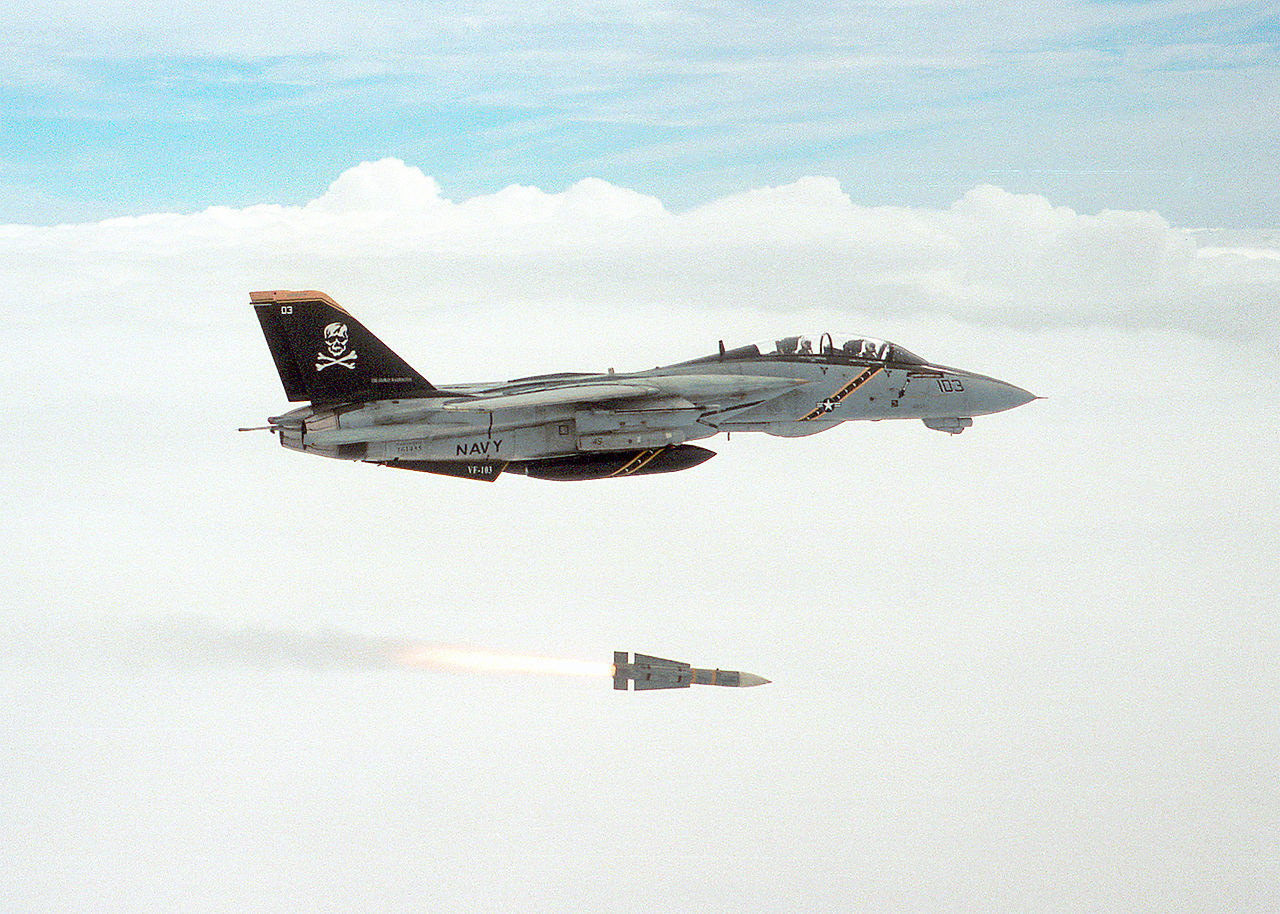
\includegraphics[width=0.6\textwidth]{phoenix.jpg}
	\caption{照片由美国海军上尉 Dana Potts 拍摄 (020924-N-1955P-001)}
\end{figure}

AIM-54 远程空空导弹和F-14“雄猫”一起诞生于当年的TFX项目。

最初为 F-111B 设计的 AIM-54 被 F-14 用作可以同时攻击敌方轰炸机和巡航导弹的长射程导弹。当然,AIM-54 打击其他小目标也并非力不从心。

AIM-54 导弹最突出的特点便是超远的射程。AIM-54 还具有同时发射和跟踪最多6个目标的能力,先由载机上的 AN/AWG-9 雷达制导,然后用自己的主动雷达引导头独立制导。

AIM-54 最初的型号是安装 Mk47火箭发动机的 AIM-54A。Mk47 发动机后来升级为 Mk60 火箭发动机以增加导弹的射程。而 AIM-54 本身也经过升级成为 AIM-54C,改进的引导头引导能力更强,新的 Mk47 发动机发烟量也更少,更难被目视发现。

美国海军在实战中仅发射了3枚 AIM-54 导弹,均于伊拉克上空发射。3枚导弹都没有击中目标,其中2枚由于火箭发动机失效,第三枚则是目标自己掉头逃跑而未能命中。

不为西方所知的是,IRIFA则宣称使用 AIM-54 对伊拉克的米格-21、米格-23、米格-25、幻影F-1和超军旗等飞机获得了至少78次空中胜利,战果甚至还包括了数枚反舰巡航导弹。

\section{一般规格}

\begin{table}[htb]
	\centering
	\caption{F-14B 技术资料}
	\begin{minipage}[t]{0.8\textwidth}
		\begin{tabularx}{\linewidth}{|l|X|X|X|X|}
			\hline
			翼展(机翼完全展开) & 64'1.5"(约19.5米)               \\
			\hline
			翼展(空中完全后掠) & 38'2.5"(约11.6米)               \\
			\hline
			翼展(停放机翼后掠) & 33'3.5"(约10.1米)               \\
			\hline
			长度                 & 62'8.5"(约19.1米)               \\
			\hline
			高度                 & 16' (约4.9米)                   \\
			\hline
			翼面积               & 565平方英尺(约52.5平米)         \\
			\hline
			空重                 & 41,780磅(约19,000千克)          \\
			\hline
			最大重量             & 74,349磅(33,700千克)            \\
			\hline
			加力最大推力         & 60,400磅力(268千牛顿)           \\
			\hline
			翼载                 & 94磅/平方英尺(458.9千克/平方米) \\
			\hline
			极速                 & 1,544英里/小时(~2,500千米/小时) \\
			\hline
			升限                 & 53,000+英尺(~16,200米)          \\
			\hline
			航程                 & 2,050海里(~3,800千米)           \\
			\hline
		\end{tabularx}
	\end{minipage}
\end{table}
